%Chapter of Implementation
%What my app has, (how it evolved?) in terms of physical structure and technologies involved

\chapter{Implementation}
\label{imple}

\section{Overview}

The Arduino Due asks for the server's new public key and for a new nonce that it should use for the following temperature data transmission. It does this by sending a GET request to a JSP page on the server. The public key and nonce are newly generated by the server and the nonce is encrypted using the keys and nonce used in the previous transmission. The Due is connected to the DS18S20 temperature sensor and it receives the temperature data over the OneWire protocol. This data is signed using the Arduino's secret signature key and then encrypted using the Arduino's secret key, the Server's new public key and the new nonce. The encrypted data is sent as a POST request to the add.php file on the apache server which executes it and the first thing add.php does is call connect.php which has the SQL database details and makes a connection to the database. Following that add.php builds up a SQL query that inserts the values sent in the post request into the appropriate table entries and then the connection is closed.
When a user want to view the files, they use a browser to send a GET request to the Java web app. The app builds up a SQL query to take out all the values from the database, decrypts them and verifies the signature before printing out in a table.
When it comes to public key transmission the Due sends a POST request to the Arduino Uno that is set up as a web server. The Uno recognises that it is receiving a POST request and stores the key.


\subsection{Temperature reading}

The DS18S20 temperature sensor is wired up with a 4.7$\Omega$ pull up resistor, between the orange wires, on the bread board shown in figure \ref{fig:tempcircuit}. A pull up resistor is a resistor between the sensor and the positive power supply so that the signal will be a valid logic level if external devices are disconnected or a high impedance is introduced. It is connected to digital pin 9, yellow wire, because it can't be on pins 10, 11, 12, 13 as they will be used by the Ethernet Shield. When looking at the temperature sensor the furtherest left pin is V$_{dd}$ and normally this would be connected to the Arduino's 3.5v or 5v output but the DS18S20 is in parasite power mode which scavenges power off the middle data line, DQ. When the DQ pin is high some of the charge is stored in a capacitor that will be used to power the device when the data is being read. In parasite power mode both the GND and V$_{dd}$ are connected together, by the bluewire, and then to ground.

\begin{figure}[H]
	\centering
	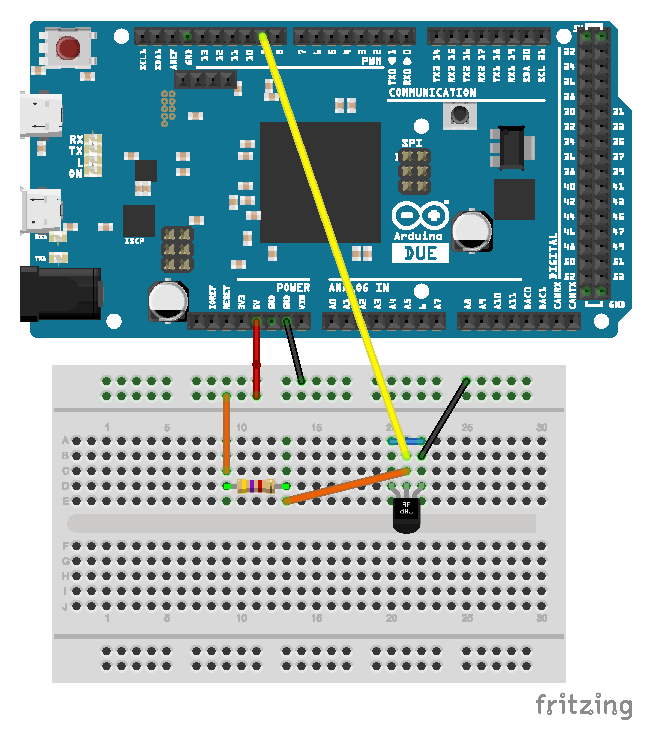
\includegraphics[width=.5\linewidth]{Figures/TempSensor_bb.pdf}
	\caption{DS18S20 in parasitic power mode connected to Arduino}
	\label{fig:tempcircuit}
\end{figure}

%can explain full scratchpad memory, CRC, or hex to int conversion
The DS18S20's scratchpad memory is divided up into 9 bytes as shown in figure \ref{fig:dsmem}. The first two bytes are the ones of most interest as they store the actual temperature value. Bytes 2 and 3 are the high and low trigger registers, these can be used to trigger some action when the temperature goes above or below a certain threshold. Bytes 4 and 5 are only for internal use and cannot be overwritten. Bytes 6 and 7 can be used to calculate the extended resolution. Byte 8 holds the cyclic redundancy check which is an error detecting technique. The bytes with asterisks are values which stored in non volatile EEPROM, the rest are stored on volatile SRAM\cite{dsdatasheet}.

\begin{figure}[H]
	\centering
	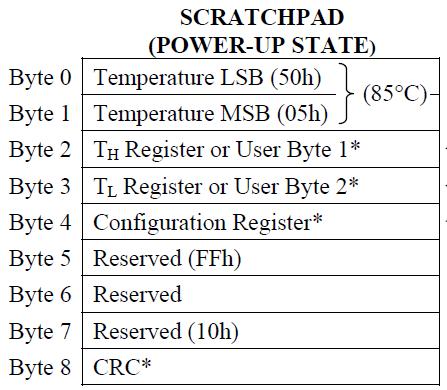
\includegraphics[width=.6\linewidth]{Figures/dsmem.png}
	\caption{DS18S20's memory organisation}
	\label{fig:dsmem}
\end{figure}

The library used to read the DS18S20 is OneWire, which is a proprietary library from Maxim that performs half-duplex bidirectional communications between a host/master controller and one or more slaves. As seen in the following code snippet, figure \ref{snip:tempcode}. The command \emph{ds.write(0x44, 1)} starts the internal A-D conversion operation. Once this process is finished the data is copied to the Scratchpad registers. A delay is needed to charge the capacitor and to ensure conversion is complete before reading the data. Which is done with \emph{ds.write(0xBE)} and then the data is read out using \emph{ds.read()} and put into an array.

\begin{figure}[H]
\begin{lstlisting}[style=Arduino]
  							OneWire  ds(9);
								...
  							ds.write(0x44, 1); 
  						 	delay(1000);

  							present = ds.reset();
  							ds.select(addr);    
 							ds.write(0xBE)

  							Serial.print("  Data = "); 
  							Serial.print(present, HEX);
 						 	Serial.print(" ");
  							for ( i = 0; i < 9; i++) {          
    								data[i] = ds.read();
    								Serial.print(data[i], HEX);
    								Serial.print(" ");
  							}

\end{lstlisting}
\caption{DS18S20 temperature sensor Arduino Code}
\label{snip:tempcode}
\end{figure}


\section{Cryptographic}

Before the data can be signed and encrypted the new nonce and server public key have to be requested. The Due sends a GET request in a very similar manner to the POST request shown in figure \ref{snip:ethernet} and the server returns, byte by byte, the information. The Arduino takes the char arrays and converts them into two byte array. The public key is sent unencrypted so a human user must check that it is the same key in this demo application but the nonce is sent encrypted and signed. Shown in figure \ref{snip:denonce} if this is the first transmission then the nonce will have been encrypted using the presintalled keys and nonce else the server public key nonce and generated by the server previously are used. The way the Arduino knows if this is the first transmission is if the byte array \emph{serverpkold} is empty as after the temperature data is encrypted the old nonce and server public key and stored in another array so they can be used to decrypt the next nonce. Throughout this application the same signatures are used. The Due decrypts the nonce using the relevant keys and removes the 32 bytes of leading zeros that needed to be placed by the server for successful encryption before verifying the signature in line 12. Nonces are 24 bytes in length and a signature is 64 bytes in length.

\begin{figure}[H]
\begin{lstlisting}[style=Arduino]
#include <TweetNaCl2.h>
TweetNaCl2 tnacl;
int Suc_Decrypt;
int Suc_SignVerify;
int scnlenwz = crypto_box_NONCEBYTES + crypto_sign_BYTES + crypto_box_ZEROBYTES; 
byte scnoncenewtemp[scnlenwz]; //signed encrypted nonce with zeros
byte snoncewz[scnlenwz]; // signed nonce with zeros
int snlenwoz = crypto_box_NONCEBYTES + crypto_sign_BYTES;
byte snoncewoz[snlenwoz]; //signed nonce without zeros
int snlen = crypto_box_NONCEBYTES;
byte nonce[snlen];
	...
if(serverpkold[0]==NULL){
	Suc_Decrypt = tuit.crypto_box_open(snoncewz, scnoncenewtemp, scnlenwz, preinstallnonce, preinstallserverpk, arduinosk); 
}else{
	Suc_Decrypt = tuit.crypto_box_open(snoncewz, scnoncenewtemp, scnlenwz, nonceold, serverpkold, arduinosk);
}

Suc_SignVerify = tuit.crypto_sign_open(nonce,&nlen,snoncewoz,snlenwoz,serverpksign);

\end{lstlisting}
\caption{Decrypting the next nonce}
\label{snip:denonce}
\end{figure}

Now that the server public key and nonce have been found the secure temperature data transmission can take place. Much like the server, when the Arduino is encrypting a signature and message it must have padded out the data with 32 bytes of leading zeros specified in the NaCl website. Take special care that exactly 32 bytes are placed in front because if there isn't the correct number the encryption process will still complete without errors. However the decryption will fail and it isn't apparent that that error occurred when data was encrypted. The code used to sign and encrypt the data is shown in figure \ref{snip:nacl}.

\begin{figure}[H]
\begin{lstlisting}[style=Arduino]
#include <TweetNaCl2.h>
TweetNaCl2 tnacl;

byte arduinosk[crypto_box_SECRETKEYBYTES] = {...};
byte arduinosksign[crypto_sign_SECRETKEYBYTES] = {...};
byte serverpk[crypto_box_PUBLICKEYBYTES]  = {...};
byte nonce[crypto_box_NONCEBYTES] = {...};

int const messageLength = crypto_sign_BYTES + 9;
byte message[messageLength] = {...};
unsigned long long signedMessageLength=0;
byte signedCipher[signedMessageLength];
unsigned char signedMessage[messageLength+crypto_sign_BYTES];

tnacl.crypto_sign(signedMessage, &signedMessageLength, message, messageLength, arduinosksign);
tnacl.crypto_box(signedCipher, signedMessage, signedMessageLength, nonce, serverpk, arduinosk);
\end{lstlisting}
\caption{TweetNaCl Arduino Signature and Encryption Code}
\label{snip:nacl}
\end{figure}

The C TweetNaCl library has been converted into an Arduino library. The Arduino lanugage is based on C and C++. It therefore needs an instance of TweetNaCl created which in the sketch is called \emph{tnacl}. With this instance the methods needed can be accessed. In this prototype some keys are preinstalled, the Arduino's secret key, it's secret signature key, the server's public signature key and the first nonce and first server public key that will only be used once to decrypt the first nonce. With each transmission the Due will get a new nonce and server public key. 

Lines 4-13 set up the message byte arrays that are to be passed between the methods. \emph{message} is initialised as a byte array of size \emph{messageLength} which can has to be \emph{crypto\_box\_ZEROBYTES}, 32 bytes, plus the length of the message. \emph{signedMessage} and \emph{signedMessageLength} are passed in by reference so after \emph{crypto\_sign()} is complete the message with the signature and the size of that array will be in those variables, respectively. The resulting signed message needs to have 32 bytes of leading zeros added to it before encryption. The function \emph{crypto\_box} completes that takes and the places the cipher into \emph{signedCipher} which is passed in by reference. 

\clearpage

\section{Data transmission}
Once the data has been encrypted it is to be packaged up and sent across the network.

\begin{figure}[H]
\begin{lstlisting}[style=Arduino]
#include<Ethernet2.h> //Ethernet Shield R2 library
#include<SPI.h>

byte mac[] = {
0x90, 0xA2, 0xDA, 0x10, 0x2D, 0xD6 //of the Ethernet Shield
};
char server[] = "192.168.0.6"; //IP of apache web server
EthernetClient client;

IPAddress clientIP(192, 168, 0, 30);

 if(Ethernet.begin(mac)==0){
      Serial.println("Failed to assign IP");
      Ethernet.begin(mac, clientIP);
  }else{
     Serial.println("Assigned IP");
  }

if(client.connect(server,80)){
     String data = "temperatureHex=";
     int contentLength = data.length()+final.length();
     Serial.println("Connected");   
     client.println("POST /tempLog/add.php HTTP/1.1"); 
     client.println("HOST: 192.168.0.6"); 
     client.println("Content-Type: application/x-www-form-urlencoded");
     client.print("Content-Length: ");
     client.println(contentLength);
     client.println();
     client.print("temperatureHex=");
     client.print(final);
   }else{
       Serial.println("Failed to Connect");
   }
   
   client.stop();
\end{lstlisting}
\caption{Ethernet interfacing and transmission Code }
\label{snip:ethernet}
\end{figure}
 Just before the cipher is sent the byte array is converted into a String so that it can be passed around easily as one parameter. This is completed simply by cycling through the byte array and adding each entry together. Care has to be taken when there are hexadecimals that are 0x0F or lower. The leading zero is lost during the conversion to String which means that when the cipher reconverted into a byte array, it is incorrect and cannot be decrypted. This is solved by explicitly adding an extra ``'0'' String if the byte is less than or equal to 0x0F.  The device needs an IP address which is completed through Dynamic Host Configuration, DHCP by the router. The router running DHCP dynamically allocates network configuration parameters such as IP addresses to devices so that they automatically get one that isn't in use. This is completed with the line \emph{Ethernet.begin(mac)} which returns a 1 on successful IP allocation or 0 on failure. If it fails then a static IP can be assigned manually by \emph{Ethernet.Begin(mac, clientIP)}. A connection to the server is attempted using the IP and the port number, 80 in this case. If it successful the information is transmitted as a POST request, a POST request is a request method in the HTTP protocol. When a server receives a POST request it knows to take the data and complete an action with it. The request makes it known that it wants add.php to be executed upon receiving the data. %extra params, the content size and urlencoding
Once the data is sent the connection can be closed and other actions performed on the Arduino.
 
\section{Server Side}

For the prototype, an Apache and Tomcat server with SQL was set up using XAMPP on a desktop. The Arduino causes the add.php to be run and the first thing that it does is make a connection to the SQL server using SQL IP address, username, password and the name of the database. If it can't connect it abandons the task and returns an error message. On successful connect it returns the connection variable.

\begin{figure}[H]
%\begin{lstlisting}[language=PHP]
\begin{lstlisting}[style=PHP]
<?php
   	include("connect.php");
 
   	$link=Connection();
	
	$temp=$_POST["temperatureHex"];
 
	$query = "INSERT INTO tempLog (tempHex) 
		VALUE ('".$temp."')"; 
 
   	mysql_query($query,$link);
   	mysql_close($link);
 
   	header("Location: index.php");
?>
\end{lstlisting}
\caption{Arduino to SQL interfacing code}
\label{snip:php}
\end{figure}

The data to be stored is extracted out of the POST request and placed in a variable. Then an SQL query is built up before being sent to the SQL server and the connection terminated. The SQL table contains an ID, the time at which the temperature data was received and the data and is created using the command shown in figure \ref{snip:sql}. Notice between the database creation code and the PHP file the corresponding variables, tempLog, the table name and tempHex, the data.

\begin{figure}[H]
\begin{lstlisting}[style=SQL]
CREATE TABLE `iotplatform`.`tempLog` ( `id` INT(255) NOT NULL AUTO_INCREMENT , `timeStamp` TIMESTAMP on update CURRENT_TIMESTAMP NOT NULL DEFAULT CURRENT_TIMESTAMP , `tempHex` VARCHAR(100) NOT NULL , PRIMARY KEY (`id`)) ENGINE = InnoDB;
\end{lstlisting}
\caption{SQL database creation code}
\label{snip:sql}
\end{figure}
%InnoDB?

The data stored in the database is still encrypted, now a way is needed to decrypt it and display it to the user. A Java web app, using Java server pages, JSP, was created as there are Java implementations of the TweetNaCl library, among other variations, available\cite{ian}. Eclipse JEE Mars was used to create a dynamic web project which extends HttpServlet for the creation of dynamic web pages. In this you override at least one of the following methods, doGet, doPost, doPut and doDelete so depending on the type of request received a different action will occur. This application has the code in the doGet as the server will receive a get request when it is accessed by a user.

\subsection{Decryption and display of temperature data}

\begin{figure}[H]
\begin{lstlisting}[style=Java]
protected void doGet(HttpServletRequest request, HttpServletResponse response) throws ServletException, IOException {
response.setContentType("text/html");
PrintWriter printWriter  = response.getWriter();
printWriter.println("<html>");
}
\end{lstlisting}
\caption{Prepping the client printer in JSP}
\label{snip:clientprinterjsp}
\end{figure}

Using the code shown in figure \ref{snip:clientprinterjsp} the headers and tags you would need and expect in a HTML page can now be printed dynamically much like printing to a console. The keys are defined similarly to the code on the Arduino except the server has it's own secret key and the Arduino's public key.

\begin{figure}[H]
\begin{lstlisting}[style=Java]
	final String DB_URL="jdbc:mysql://localhost/iotplatform";
	String user = "root"; 
	String password = "";
	try
	        {
	          // Register JDBC driver
	          Class.forName("com.mysql.jdbc.Driver").newInstance();

	            // Open a connection
	            Connection conn = DriverManager.getConnection(DB_URL, user, password);

	            // Execute SQL query
	            Statement stmt = conn.createStatement();
	            String sql;
	            sql = "SELECT id, timeStamp, tempHex FROM tempLog";
	            ResultSet rs = stmt.executeQuery(sql);
	            // Extract data from result set
	            while(rs.next()){
	               //Retrieve by column name
	               int id  = rs.getInt("id");
	               String tempHex = rs.getString("tempHex");
	               Timestamp timeStamp = rs.getTimestamp("timeStamp");
	}
}
\end{lstlisting}
\caption{Accessing the SQL database in JSP}
\label{snip:jspcode}
\end{figure}

In figure \ref{snip:jspcode} is a section of code running in tomcat. The java application was created with Eclipse Mars and was exported as a WAR file before being store in the tomcat directory. The app is given the SQL details before entering a try catch that prints whatever the error message is to the client. Java database connectivity, JDBC, is an API for client access to a database. Before the java app is exported as a WAR file it must have the JDBC bin jar in the lib folder in WEB-INF for the eclipse project otherwise this won't work. The app gets a new instance of JDBC and then opens a connection to the server before building up a query to pull out the contents of the table. The variables are put into a result set which can be used to access each individual variable with the string name as a parameter. The encrypted message is still in it's String format and needs to be converted back into a byte array. During the conversion to a String on the Arduino half of the leading zeros are lost but they are added again before the conversion to byte array. The API in the Java implementation of is compatible with the TweetNaCl C API but provides another level of abstraction on top. 

\begin{figure}[H]
\begin{lstlisting}[style=Java]
TweetNaCl.crypto_box_open(signedMessage, cipher, messageLength, nonce, arduinoPublicKey, serverSecretKey);
byte[] javaPlainTextMessage = TweetNaCl.crypto_sign_open(signedCipherArray, ArduinoPublicSignatureKey);
\end{lstlisting}
\caption{Decryption of message and verification of signature in JSP}
\label{snip:decryptjsp}
\end{figure}

The security needs to be taken open in the reverse order as to how it was put on. The nonces and secrets keys used have been stored in the order they were created. Which corresponds with the order of the data in the SQL database. As each entry from the table is removed the corresponding secret key and nonce , from the 2D arrays, is used. \emph{TweetNaCl.crypto\_box\_open} passes the decrypted message out by reference but for \emph{TweetNaCl.crypto\_sign\_open} the message without the signature is returned. This is an example of the top layer of abstraction in Ian Preston's implementation of TweetNaCl. The  \emph{TweetNaCl.crypto\_box\_open} method is the exact same as the the C library but \emph{TweetNaCl.crypto\_sign\_open} is a slightly built upon method that has fewer parameters, completes more work behind the scenes and returns the byte message. The variable \emph{javaPlainTextMessage} is the temperature in plain hexadecimal but it still needs conversion to integer so it can be read by the average user. The code is taken from the DS18S20 example from Arduino.

The web app upon being accessed decrypts and checks the signature of each entry, using the keys that it has stored, in the table before converting the raw hex temperature data into more readable integers and displaying in a simple HTML table that can be accessed by the user. When the Arduino has data to send it will make a POST request to a PHP file on the Apache server which takes the data given to it and places it in the SQL server.

\section{Encrypted Nonce transmission}
A new nonce needs to be created for each new communication. This is done using Java's psuedo random number generator from the class Random. This new random nonce is stored in a 2D array in the web application so that the application can decrypted and display the data later. Then it is signed with the server's signature, which doesn't change in this application. If this is the first transmission and therefore the first public key and nonce to be produced, the nonce with signature is encrypted using the presintalled keys otherwise it will use the secret key and nonce created in the previous transmission. The encrypted nonce is printed out to the Due with two terminating characters either side.

\section{Public Key Transmission}
\label{pktransmit}

For a secure connection public keys must be sent. At the start of the Arduino due's code it sent a GET request, very similar to the POST request shown in figure \ref{snip:ethernet}. The request is sent to a Java page called Secret Key. This page is similar in set up to the page a user accesses to view the temperature data. When accessed the page calls \emph(TweetNaCl.crypto\_box\_keypair()) to create the server's secret key and corresponding public key and the public key. It stores the secret key in a 2D array and prints out the public key to the Due with two terminating characters either side. Along with the next nonce, this process is explain in section \ref{nonce} Once this request has been sent the server sends all of the information, byte by byte. Which also includes information about the server, data and time. During debugging this can be used to print out the state of the web application as it is being run. The code used to extract the the public key is very similar to the code shown in figure \ref{snip:post} expect it watches for the character < to signify that the next word will be the key. Afterwards the key needs to be converted back into a byte array from string before it can be used. The key is then used to encrypt the next temperature data transmission before being copied over into a second array so that it can be used to decrypt the nonce that will be sent encrypted from the server for the next secure temperature data transmission. 

For the creation of other nodes on the network that are connected onto the Due, an Arduino Uno was set up as a host and example node. As two clients can't directly connect together with the Ethernet protocol and since the Arduino Due is a client to a web server, the Uno must be a host. The Uno will be a server similar to the XAMPP web server expect it isn't directly connected to the internet. 
The Due sends a POST request to the Uno, very similar to the one it sends to the XAMPP web server, in figure \ref{snip:ethernet} however the key is under the content header. The method that the Due uses, sending a POST request that executes a php file to extract the data from the POST cannot be used, without difficulty??, as PHP can't be run on an Arduino web server. Instead there is an extra header in the POST, \emph{``Content: key''}.

\begin{figure}[H]
\begin{lstlisting}[style=Arduino]
String incomingWord = " ", key = "";
int saveNextWord = 0, takeData = 0;
 if (client.available()) {
        char c = client.read();
        Serial.write(c);
        if(c == ' '){
          key = incomingWord;
          incomingWord=" ";
        }else{
          incomingWord = incomingWord + c;
        }
        if((incomingWord=="Content") && (takeData)){
           saveNextWord = 1; 
        }
        if(incomingWord=="POST"){
          takeData=1;
        }
}
\end{lstlisting}
\caption{Handling POST requests in Arduino}
\label{snip:post}
\end{figure}

When setting up the Uno server, explicitly define what gateway and subnet the router being used has as the defaults \emph{Ethernet.begin(mac)} uses aren't always correct. The server sits open on a certain port, 8081 in this case, and waits for clients to make a connection. Once they have, the server sends an acknowledgement that it has received a connection and starts reading in the request. There it watches out for the word POST so that it knows to store the content and, of course, for the content so it knows what to store. The request from the client is read out a byte at a time so it is necessary for those bytes to be made into strings so specific keywords can be looked out for. If the byte is not a space then it is part of a word so it is added to the subsequent bytes until another space is reached then it is considered a word and compared against. Once the key is taken it is in String format and needs to be turn back into hex and store as the key to be used in further encryptions.


\section{TweetNaCl Library}

The TweetNaCl library as it stands in it's original form is not compatible with Arduinos. The C library compiles without errors but the compiler warns that the TweetNaCl method names are undefined and as a result do not perform their tasks. The Arduino language is a mix of C++ and C so it doesn't support every aspect of each language. When the methods are accessed they simply returns random numbers, it is possible that it is trying to access some area of memory, not finding the correct function and simply returning whatever it finds. It is not understand why this is the case but to get the libraries to work it is a simple case of converting the library into C++ syntax. With a header file that has the main methods used in the project and the \#defines and a cpp file with the TweetNaCl code. This is added in the same way to the Arduino IDE and in the code an instance of the class is created and methods are accessed with the dot operator. In this application not every function in the TweetNaCl library will be used so any methods that weren't going to be utilised were not copied over into the converted library.



